\section*{Implementation:}\label{sec:implementation}

%%%%%%%%%%%%%%%%%%%%%%%%%%%%%%%%%%%%%%%%%%%%%%
% ESP-Now Mesh (SLAVE) - Ben
%%%%%%%%%%%%%%%%%%%%%%%%%%%%%%%%%%%%%%%%%%%%%%
\subsection{ESP-Now Mesh}\label{sec:espnowmesh}

%%%%%%%%%%%%%%%%%%%%%%%%%%%%%%%%%%%%%%%%%%%%%%
% LORA Mesh (SLAVE) - Richie
%%%%%%%%%%%%%%%%%%%%%%%%%%%%%%%%%%%%%%%%%%%%%%
\subsection{LORA Mesh}\label{sec:loramesh}

%%%%%%%%%%%%%%%%%%%%%%%%%%%%%%%%%%%%%%%%%%%%%%
% Master Node Stack
%%%%%%%%%%%%%%%%%%%%%%%%%%%%%%%%%%%%%%%%%%%%%%
\subsection{Master Node Infrastructure}\label{sec:master}

The Master Node Infrastructure encompasses a suite of pivotal components meticulously designed to harmoniously facilitate the monitoring and management of IoT devices. Charged with duties spanning data aggregation, processing, and user interface provisioning, the Master Node assumes a central role in orchestrating system functionalities. Core elements of this infrastructure comprise the Liligo Gateway, a Raspberry Pi MQTT Client and Broker, and the ELK Stack. Furthermore, our implementation integrates a router to establish an artificial cloud-based server for the ELK Stack.

\subsubsection{Protocol Master}\label{sec:protocol}

Serving as the protocol master within the Master Node setup, the Liligo Module shoulders the vital responsibilities of traffic monitoring, serialization, and MQTT-based transmission to the ELK stack. In collaboration with a Raspberry Pi configured as both MQTT Client and Broker, the Liligo Module establishes a USB connection for seamless data transfer to the Raspberry Pi. Subsequently, the Raspberry Pi orchestrates the dissemination of serialized data to the ELK stack via MQTT.

Configured to monitor Lora and ESP-Now Protocol packets, the Liligo Module acts as the primary data acquisition unit. Upon reception, data undergoes serialization and is then forwarded to the MQTT Broker by the Raspberry Pi 4b, facilitating streamlined integration with the ELK stack for subsequent processing.

\subsubsection{ELK Stack}\label{sec:elk}
% Backbone Cloud-based server Stack
\begin{figure}[h]
  \begin{center}
    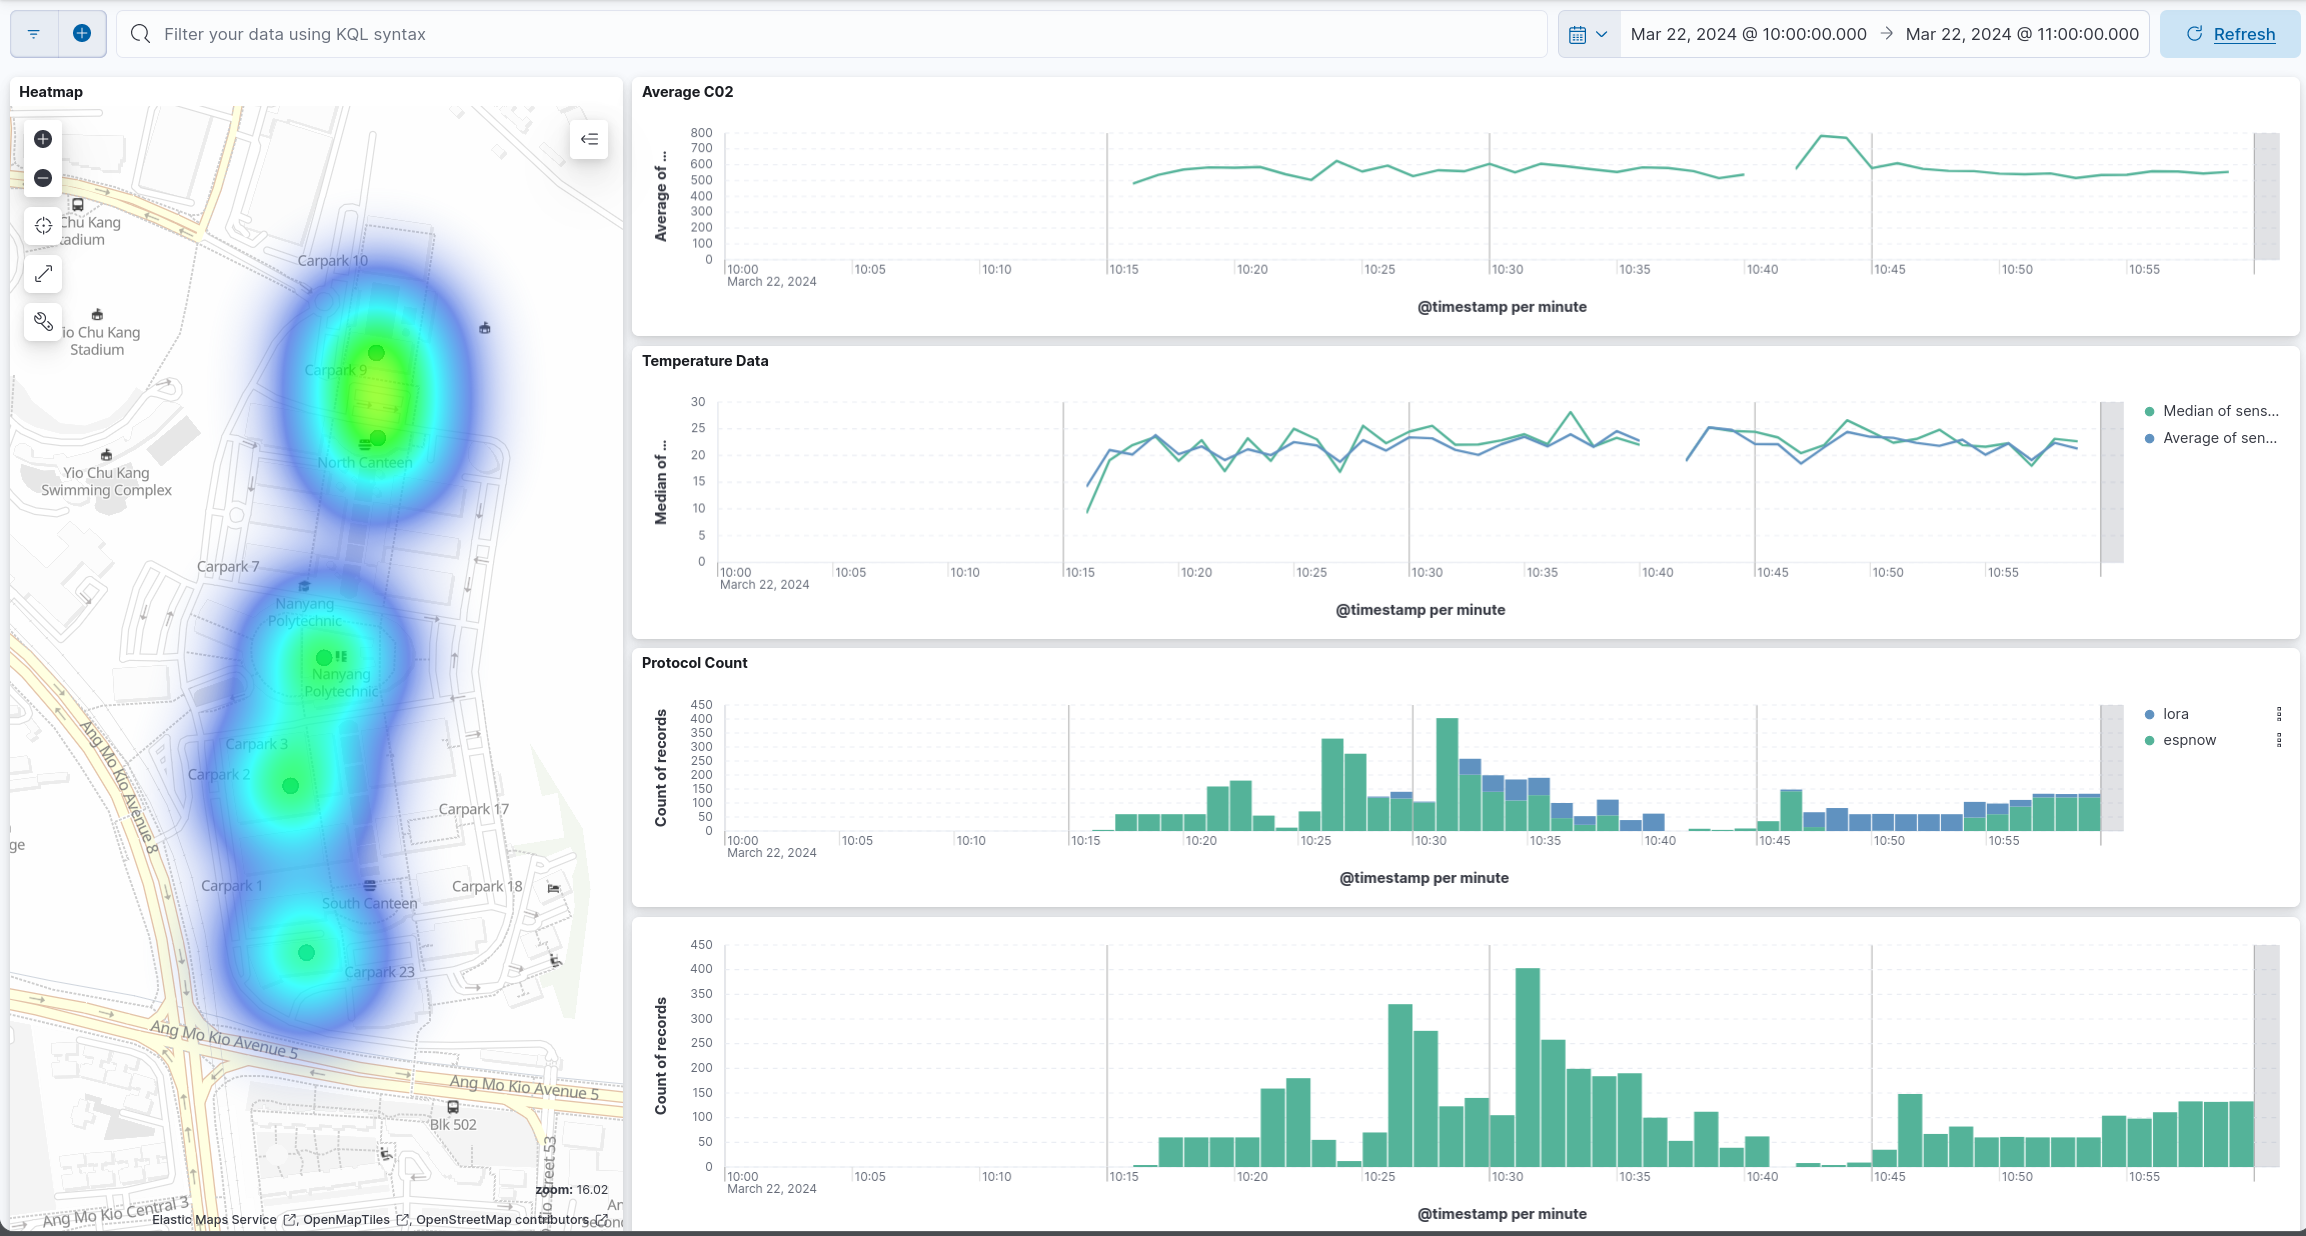
\includegraphics[width=0.35\textwidth]{./Figures/elk/elk_dashboard.png}
  \end{center}
  \caption{ELK Dashboard}\label{fig:elk_dashboard}
\end{figure}

The deployment of the ELK Stack is streamlined through the utilization of Docker and Docker Compose, enabling efficient deployment with minimal configuration overhead. Comprising Elasticsearch, Logstash, and Kibana, the ELK Stack offers a robust framework for data storage, processing, and visualization. Elasticsearch, a distributed, RESTful search and analytics engine, serves as the cornerstone for storing extensive datasets. Logstash functions as a versatile data processing pipeline, ingesting data from diverse sources, transforming it, and then forwarding it to a designated "stash" such as Elasticsearch. Kibana, a powerful data visualization dashboard, empowers users to interact with and explore data stored in Elasticsearch.

Raw data emanating from the Liligo Module is routed to the Raspberry Pi before being relayed to the ELK stack for processing. Following processing, data is stored within Elasticsearch. Kibana is subsequently employed to create visualization dashboards, offering insights into various metrics such as packet transmission, environmental parameters, device connectivity, and protocol distribution.

These visualizations furnish valuable insights facilitating the monitoring of the Wireless Sensor Network (WSN), enabling performance evaluation of protocol switching. This analysis, outlined in Section \ref{sec:analysis}, encompasses metrics including packet transmission, environmental data, device connectivity, protocol distribution, and power consumption analysis.

\subsubsection{Switching}\label{sec:switching}

A pivotal feature ingrained within all slave nodes is the capability to seamlessly transition between the LORA and ESP-Now protocols in response to evolving network dynamics. This feature assumes paramount significance in the comprehensive evaluation of each protocol's efficacy across diverse network conditions. The switching mechanism, autonomously activated by individual slave nodes, predicates its decision on the observed packet failure rate. Upon discerning a notable uptick in packet failures, the slave node instigates a judicious transition to the alternative protocol. Such a mechanism stands as a linchpin in preserving network robustness and fostering optimal performance amidst fluctuating network exigencies.

An inherent advantage of this mechanism lies in its facilitation of comparative performance assessments between the two protocols amidst varying network topologies and conditions. By juxtaposing their respective performance metrics, stakeholders can glean invaluable insights into the aptness of each protocol for specific application scenarios contingent upon the prevailing network milieu. Moreover, the dynamic switching functionality serves as a potent tool for pinpointing the protocol best suited to a given network configuration, thereby engendering heightened network efficiency and reliability.


%%%%%%%%%%%%%%%%%%%%%%%%%%%%%%%%%%%%%%%%%%%%%%
% Analysis
%%%%%%%%%%%%%%%%%%%%%%%%%%%%%%%%%%%%%%%%%%%%%%
\section*{Analysis}\label{sec:analysis}

\subsubsection{Bandwidth Comparison}\label{sec:bandwidth_comparison}
% JW
% Get numbers from Dashboard + Images
\begin{figure}[h]
  \begin{center}
    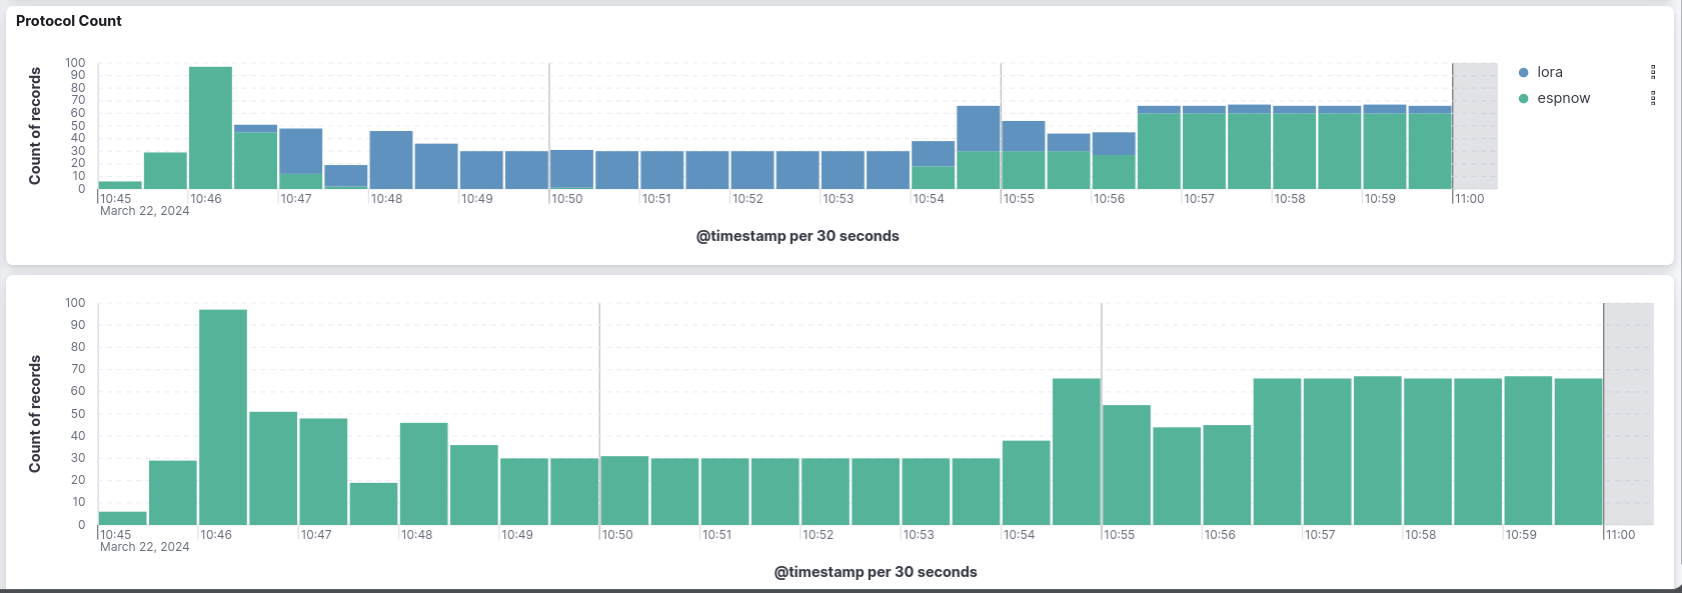
\includegraphics[width=0.45\textwidth]{./Figures/elk/protocol_count.png}
  \end{center}
  \caption{Protocol Distribution}\label{fig:protocol_distribution}
\end{figure}

Figure \ref{fig:protocol_distribution} delineates the distribution of transmitted packets across the Lora and ESP-Now protocols. The graph portrays Lora Packets denoted in blue and ESP-Now Packets in green. Evidently, the ESP-Now protocol emerges as the predominant choice, exhibiting a higher packet count vis-à-vis the Lora protocol.

The discernible instances of protocol switching, notably observed around the timestamps 10:46 and 10:54, underscore the dynamic nature of the implemented ESP-Now Mesh and LORA Mesh. During these transitions, a shift from Lora to ESP-Now and vice versa is perceptible, as delineated by the transitions between the blue and green segments in the graph.

An intriguing observation pertains to the periodic dips in bandwidth, indicative of intervals where the network experiences a diminished packet reception rate. Plausible factors contributing to this phenomenon encompass variances in protocol efficiency or disparities in mesh implementation. Despite both protocols being instantiated with the DSR mesh algorithm, the Lora protocol potentially suffers from a lower packet reception rate owing to its inherent characteristics, including a lower data rate and extended transmission range.

\subsubsection{Power Analysis}\label{sec:power_analysis}
% Jovian
